\documentclass[review]{elsarticle}

%% Use the option review to obtain double line spacing
%% \documentclass[authoryear,preprint,review,12pt]{elsarticle}

%% Use the options 1p,twocolumn; 3p; 3p,twocolumn; 5p; or 5p,twocolumn
%% for a journal layout:
%% \documentclass[final,1p,times]{elsarticle}
%% \documentclass[final,1p,times,twocolumn]{elsarticle}
%% \documentclass[final,3p,times]{elsarticle}
%% \documentclass[final,3p,times,twocolumn]{elsarticle}
%% \documentclass[final,5p,times]{elsarticle}
%% \documentclass[final,5p,times,twocolumn]{elsarticle}

\usepackage{hyperref}
\usepackage{amsmath}
\usepackage{amssymb}
\usepackage{braket}
\usepackage{siunitx}
\usepackage[version=4]{mhchem}
\usepackage{tikz}
\usetikzlibrary{positioning}
\usetikzlibrary {arrows.meta} 
\usepackage{paralist}
\usepackage{todonotes}

\DeclareMathOperator{\erf}{erf}

%% The lineno packages adds line numbers. Start line numbering with
%% \begin{linenumbers}, end it with \end{linenumbers}. Or switch it on
%% for the whole article with \linenumbers.
%\usepackage{lineno}

\journal{Journal of Molecular Liquids}

\begin{document}
	
	\begin{frontmatter}
		
		%% Title, authors and addresses
		
		\title{Solvent effects on the prediction of redox potentials: application to nitroxides}
		
		\author[1]{Pierre Beaujean\corref{cor1}}
		
		\ead{pierre.beaujean@unamur.be}
		
		\cortext[cor1]{Corresponding author}
		
		\affiliation[1]{organization={Theoretical Chemistry Laboratory, Unit of Theoretical and Structural Physical Chemistry, Namur Institute of Structured Matter, University of Namur},%Department and Organization
			addressline={Rue de Bruxelles, 61}, 
			city={Namur},
			postcode={B-5000}, 
			country={Belgium}}
		
		\begin{abstract}
			This is an abstract
			
		\end{abstract}
		
		%%Graphical abstract
		\begin{graphicalabstract}
			%\includegraphics{grabs}
		\end{graphicalabstract}
		
		%%Research highlights
		\begin{highlights}
			\item Research highlight 1
			\item Research highlight 2
		\end{highlights}
		
		\begin{keyword}
			%% keywords here, in the form: keyword \sep keyword
			
			%% PACS codes here, in the form: \PACS code \sep code
			
			%% MSC codes here, in the form: \MSC code \sep code
			%% or \MSC[2008] code \sep code (2000 is the default)
			
		\end{keyword}
		
	\end{frontmatter}
	
	% \linenumbers
	
%% main text
\section{Introduction}


The quest for efficient and sustainable energy storage solutions has intensified research into various battery chemistries. Among these, nitroxide-based batteries have attracted, since their first application in 2002 \cite{nakaharaRechargeableBatteriesOrganic2002}, significant attention due to their high theoretical capacity \cite{friebeSustainableEnergyStorage2019,ernouldNitroxidesBatteryrelatedApplications2021,keDesigningStrategiesAdvanced2023}. They are generally found, like other radical polymers, as a cathode material \cite{okaRadicalPolymersRechargeable2020a,assummaNewConductingCopolymer2020}. Beyond their application in batteries, nitroxides have been extensively studied and utilized in various fields. They serve as spin labels in electron paramagnetic resonance spectroscopy \cite{torricellaNitroxideSpinLabels2021}, as mediators for organic radical reactions and polymerizations \cite{tebbenNitroxidesApplicationsSynthesis2011,leifertOrganicSynthesisUsing2023}, in organic electronic devices \cite{jiAirStableOrganicRadicals2020,xieNitroxideRadicalPolymers2021}, and as antioxidants in biological systems  \cite{souleChemistryBiologyNitroxide2007,lewandowskiNitroxidesAntioxidantsAnticancer2017,prescottBiologicalRelevanceFree2017}.

Nitroxides are organic compounds containing the nitroxyl/aminoxyl radical functional group \cite{berlinerHistoryUseNitroxides2012}. This group can exist in three redox states: the nitroxide radical ($>$\ce{N-O^.}, also shortened in \ce{N^.} in this article), which can be oxidized to the oxoammonium cation ($>$\ce{N+=O}, abbreviated \ce{N+}) or reduced to the hydroxylamine anion ($>$\ce{N-O-}, abbreviated \ce{N-}), as depicted in Fig.~\ref{fig:states}. The remarkable stability of the nitroxide radical arises from the delocalization of the unpaired electron over the nitrogen and oxygen atoms, combined with the steric protection provided by the substituents, and environmental effects due to the interaction with solvent and ions \cite{grynovaOriginScopeLongRange2013,grynovaSwitchingRadicalStability2013}. 

\begin{figure}[!h]
	\centering
	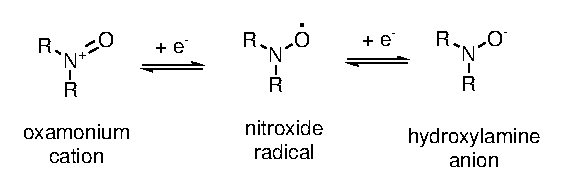
\includegraphics[width=.5\linewidth]{Figure1}
	\caption{Oxidized (left) and reduced (right) forms of the the nitroxide radical (center).}
	\label{fig:states}
\end{figure}

The performance of nitroxide-based batteries is influenced by substitents \cite{sugaCathodeAnodeActivePoly2007}, by solvation, and the nature of the electrolytes used, in particular in ionic liquids \cite{armandIonicliquidMaterialsElectrochemical2009,strehmelRadicalsIonicLiquids2012,wylieIncreasedStabilityNitroxide2019b}. Understanding the interplay between nitroxides, solvents, and electrolytes is therefore crucial for the rational design of high-performance batteries.  Computational studies using quantum chemical methods provide valuable insights into solvation effects, allowing for the prediction and tuning of redox properties. While the seminal studies of Coote and co-workers \cite{hodgsonOneElectronOxidationReduction2007,blincoExperimentalTheoreticalStudies2008} have focused on the impact of substituent on the redox potential, latter investigations by other groups have also considered the impact of electrolytes, and of the different (electrostatic, but not only) interactions between the two \cite{matsuiDensityFunctionalTheory2013,zhangInteractionsImidazoliumBasedIonic2016,zhangEffectHeteroatomFunctionality2018,wylieImprovedPerformanceAllOrganic2019a}. From a phenomenological point of view, two different approaches may be used: at low concentration in electrolytes, the Debye-Huckel (DH) theory \cite{kontogeorgisDebyeHuckelTheoryIts2018,silvaDerivationsDebyeHuckel2022,silvaImprovingBornEquation2024}  provide a first estimate for the interactions within an ionic liquid.  While improvments were proposed over the years to better consider ion-solvent interaction, especially by including dipole-ion \cite{silvaImprovingBornEquation2024} and quadrupole-ion interactions \cite{slavchovQuadrupoleTermsMaxwell2014,slavchovQuadrupoleTermsMaxwell2014a,coxQuadrupolemediatedDielectricResponse2021}, there only have been a few attempts \cite{xiaoReorganizationEnergyElectron2013,xiaoMolecularDebyeHuckelApproach2014} to include the DH theory in the prediction of redox potential  (in molten salts). However, at large concentration (such as in ionic liquids), one can expect the formation of ion-pairs \cite{marcusIonPairing2006}. Phenomenological models \cite{krishtalikElectrostaticIonSolvent1991,matsuiDensityFunctionalTheory2013,lundDielectricInterpretationSpecificity2010} (...)


Missing:\begin{itemize}
	\item Prediction of redox potential (generally, only AIP!), and \textbf{the needs for a correct description of solvent-solute interactions}
	\item So: SMD, then Debye-Huckel, then CIP (or Matsui). For that, it could be nice to do an "historic overview".
	\item Motivate the choice of water and acetonitrile and not ionic liquids (\textit{e.g.}, absence of experimental data?).
\end{itemize}

In this study, (...)

This paper is organized as follows: Section \ref{sec:theory} introduces key concepts and various simplified models that aid in the interpretation of the results. The methodology employed in this study is detailed in Section \ref{sec:methodo}. The results are then presented in four parts: the impact of substituents on the redox properties is discussed in Section \ref{sec:sar}, followed by an analysis of the effects of solvents in Section \ref{sec:solv}, and the influence of electrolytes in Section \ref{sec:elect}. Finally, a comparison between theoretical predictions and experimental results is provided in Section \ref{sec:exp}. Conclusions and future outlooks are presented in Section \ref{sec:conclusion}.

\section{Theory}\label{sec:theory}

\subsection{Redox potentials in solution}

According to Ref.~\cite{marenichComputationalElectrochemistryPrediction2014}, the absolute reduction potential $E_{abs}^0$ (in \si{\volt}) of the half-reaction of reduction of $X^z$, $X^{z} + n_e\,e^- \rightarrow X^{z-n_e}$, reads: \begin{equation}
	E_{abs}^0(X^{z}|X^{z-n_e}) = -\frac{\Delta G_{r}^\star}{n_e\,F}, \text{ with } \Delta G_{r}^\star = G^\star(X^{z-n_e}) - G^\star(X^z), \label{eq:nernst}
\end{equation}
where $\Delta G_{r}^\star$ is the free Gibbs energy of the reduction reaction in solution, $F$ is the Faraday constant (\SI{9.648533e4}{\coulomb\per\mole}) and $n_e$ the number of electrons involved in the reduction process. Last but not least, $G^\star(X^z)$ is the Gibbs free energy of $X^z$ in solution.  In the rest of this article, it is considered that $G^\star(e^-) = 0$.
The comparison between relative (vs SHE) experimental and calculated oxidation potential is performed using a common reference:\begin{equation}
	E^0_{rel}(X^z|X^{z-n_e})  = E^0_{abs}(X^z|X^{z-n_e}) - E^{0}_{abs}(\text{SHE}), \label{eq:ecalc}
\end{equation}
with $E^0_{abs}(\text{SHE}) = \SI{4.28}{\volt}$ in water or \SI{4.52}{\volt} in acetonitrile \cite{marenichComputationalElectrochemistryPrediction2014}.

From a phenomenological perspective, such $G^\star(X^z)$ values are the sum of the system's energy in vacuum, $G^0(X^z)$, and the change in (free) energy resulting from its transfer to an electrolytic solution, $\Delta G_S^\star(X^z)$. The latter can be further decomposed using the thermodynamic cycle presented in Figure \ref{fig:th}. There are four steps: $\Delta G_d + \Delta G_s$ (discharge of a sphere in the gas phase followed by charging in a dielectric) constitutes a purely electrostatic process, while $\Delta G_s$ is primarily due to non-electrostatic contributions (cavitation, van der Waals forces, etc.). Finally, $\Delta G^\star_{DH}$ incorporates the effect of surrounding ions and is therefore crucial for treating electrolytes \cite{silvaImprovingBornEquation2024}.


\begin{figure}[!h]
	\centering
	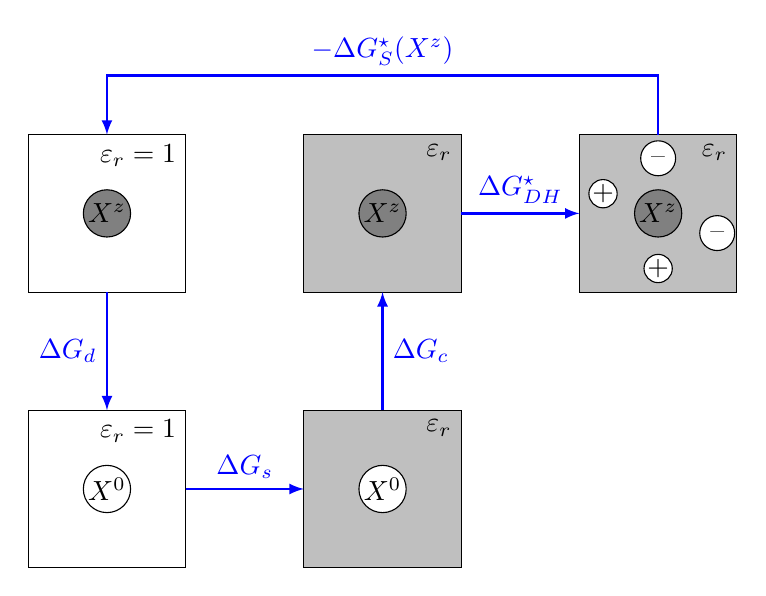
\begin{tikzpicture}
		\draw (-1,-1) rectangle +(2,2) node[anchor=north east]{$\varepsilon_r=1$};
		\draw[fill=gray] (0,0) circle (.3cm) node{$X^z$};
		
		
		\draw (-1,-4.5) rectangle +(2,2) node[anchor=north east]{$\varepsilon_r=1$};
		\draw (0,-3.5) circle (.3cm) node{$X^0$};
		
		
		\draw[fill=gray!50] (2.5,-4.5) rectangle +(2,2) node[anchor=north east]{$\varepsilon_r$};
		\draw[fill=white] (3.5,-3.5) circle (.3cm) node{$X^0$};
		
		
		\draw[fill=gray!50] (2.5,-1) rectangle +(2,2) node[anchor=north east]{$\varepsilon_r$};
		\draw[fill=gray] (3.5,0) circle (.3cm) node{$X^z$};
		
		
		\draw[fill=gray!50] (6,-1) rectangle +(2,2) node[anchor=north east]{$\varepsilon_r$};
		\draw[fill=gray] (7,0) circle (.3cm) node{$X^z$};
		\draw (2.8+3.5,-3.25+3.5) node[draw,fill=white,circle,inner sep=0]{+}
		(3.5+3.5,-2.8+3.5) node[draw,fill=white,circle,inner sep=.075cm]{--}
		(4.25+3.5,-3.75+3.5) node[draw,fill=white,circle,inner sep=.075cm]{--}
		(3.5+3.5,-4.2+3.5) node[draw,fill=white,circle,inner sep=0]{+};
		
		\draw[blue,thick,-latex] (0,-1) -- +(0,-1.5) node[midway,left]{$\Delta G_d$};
		\draw[blue,thick,-latex] (1,-3.5) -- +(1.5,0) node[midway,above]{$\Delta G_s$};
		\draw[blue,thick,-latex] (3.5,-2.5) -- +(0,1.5) node[midway,right]{$\Delta G_c$};
		\draw[blue,thick,-latex] (4.5,0) -- +(1.5,0) node[midway,above]{$\Delta G^\star_{DH}$};
		\draw[blue,thick,-latex] (7,1) -- ++(0,.75) -- node[midway,above]{$-\Delta G_S^\star(X^z)$} ++(-7,0) -- ++(0,-.75);
	\end{tikzpicture}
	\caption{Thermodynamic cycle to compute the energy of solvatation of an ion, $X^z$, in a electrolyte (solvent characterized by a $\varepsilon = \varepsilon_0\,\varepsilon_r$ dielectric constant and by a ``cloud'' of other ions). $\Delta G_d$ is the discharge of $X^z$ in gas phase, $\Delta G_s$ is the solvatation of $X$, $\Delta G_c$ is the charging of $X$ in $\varepsilon$, and $\Delta G^\star_{DH}$ is the addition of the other ions.}
	\label{fig:th}
\end{figure}


On the one hand, at the quantum chemistry (QC) level, the solvatation energy is generally treated implicitly, thanks to a self-consistent reaction field approach (SCRF) \cite{herbertDielectricContinuumMethods2021}: \begin{align}
	G^\star_{SCRF}(X) &= \Braket{\Psi|{\hat{H}+\frac{1}{2}\hat{R}}|\Psi} + G_{th}[\Psi] + G_{nonelst}(X) \nonumber\\
	&= E[\Psi] + G_{th}[\Psi] + \underbrace{G_{elst}[\Psi] + G_{nonelst}(X)}_{\Delta G^\star_{S,SCRF}(X)}, \label{eq:scrf}
\end{align}
where $\Psi$ is the wavefunction of $X$ (minimized under the application of $\hat R$, so not equal to the gas phase wavefunction), $\hat H$ is the electronic Hamiltonian, $\hat R$ is the reaction field operator (generally recognized to give rise to the electrostatic contribution to the solvation energy, $G_{elst}$), $G_{th}$ are the thermal contributions to the Gibbs free energy derived from thermostatistic analysis, and $G_{nonelst}$ is the non-electrostatic contributions (cavitation, dispersion, etc) to the solvation energy. Therefore, using the notation of Figure \ref{fig:th} (and assuming no change in the geometry of $X^z$), $ \Delta G^\star_{S,SCRF}(X^z) = \Delta G_d + \Delta G_s + \Delta G_{c}$.  

On the other hand, the Debye-Huckel (DH) theory provide another estimate of $\Delta G_{S}^\star$ \cite{bockrisModernElectrochemistryIonics1998}. Indeed, assuming that a ion $X^z$, bearing a charge $q = z\,e_0$ ($e_0$ is the elementary charge), can be approximated by a sphere of radius $a$ and that the ions in the solution are distributed in the solution according to Maxwell-Boltzmann statistics, one obtains the corresponding solvation energy as \cite{kontogeorgisDebyeHuckelTheoryIts2018,silvaDerivationsDebyeHuckel2022,silvaImprovingBornEquation2024}:\begin{align}
	\Delta G^\star_{S,DH}(X^z)
	&= \Delta G^\star_{born}(X^z) + \Delta G^\star_{DH}(X^z)\label{eq:adh}
\end{align}
where:
\begin{equation}
	\Delta G^\star_{Born}(X^z) =\frac{q^2}{8\pi\varepsilon_0\,a}\,\left[\frac{1}{\varepsilon_r}-1\right], \label{eq:born}\\
\end{equation}
and,
\begin{align}
	&\Delta G^\star_{DH}(X^z) = -\frac{q^2}{4\pi\varepsilon_0\varepsilon_r}\,\frac{\kappa}{(\kappa\,a)^3}\,\left[\ln(1+\kappa\,a)-\kappa\,a+\frac{1}{2}(\kappa\,a)^2\right],\label{eq:dh} \end{align}
in which $\kappa$ is the inverse of the Debye screening length, defined from:\begin{equation}
	\kappa^2 = \sum_i \frac{n_i\,q_i^2}{\varepsilon_0\varepsilon_r\,k_B\,T}, \label{eq:kappa2}
\end{equation}
where $n_i$ is the number density ($n_i = N_i / V = c_i\,\mathcal{N}_a$ where $\mathcal{N}_a$ is the Avogadro number and $c_i$ is the concentration in ion $i$) of ion of type $i$, $k_B$ is the Boltzmann constant (\SI{1.380649e-23}{\joule\per\kelvin}), and $T$ is the temperature (assumed to be \SI{298.15}{\kelvin}).  $\kappa$ is  proportional to the ionic strength of the solution, $I = \frac{1}{2}\sum_i c_i\,z_i^2$.  The Born part is generally dominant in solvatation energies predicted by this model (Fig.~S1).

In the limit of $\kappa\to 0$,  $\Delta G^\star_{DH} = 0$ and thus $\Delta G^\star_S \approx \Delta G^\star_{born} = \Delta G_d + \Delta G_c$.  Therefore, by combining Eqs.~\eqref{eq:scrf} and \eqref{eq:adh}, one defines:\begin{equation}
	G^\star(X^z) = G^\star_{SCRF}(X^z) + \Delta G^\star_{DH}(X^z), \label{eq:gtot}
\end{equation}
to be used in Eq.~\eqref{eq:nernst}. It should provide similar results to the approach developed by Cossi \emph{et al.} in Ref.~\citenum{cossiInitioStudyIonic1998}.

\subsection{Model for the impact of the substituent}

In a first approximation, the electrostatic interaction between the substituent(s) and the charge formed upon oxidation or reduction influences the redox potential of nitroxides. Specifically, assuming a non-charged substituent, charge-dipole interactions stabilize the oxoammonium ($>$\ce{N+=O}) if the dipole is aligned with the charge, while they destabilize the hydroxylamine ($>$\ce{N-O-}), both resulting in a decrease in the redox potential (see Fig.~\ref{fig:dipole}). Within this framework, it is therefore expected that compounds with donor substituents have lower redox potentials than acceptor substituents.


\begin{figure}[!h]
	\centering
	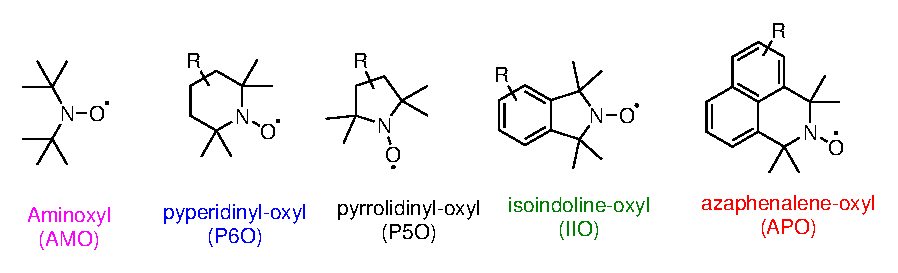
\includegraphics[width=.7\linewidth]{Figure2}
	\caption{Impact of the dipole orientation of the substituent on the redox potential when the dipole is oriented in  the positive $x$ direction (red) or not (blue). Adapted from Ref.~\citenum{zhangEffectHeteroatomFunctionality2018}.}
	\label{fig:dipole}
\end{figure}

In 2018, building upon previous work by Gryn'ova et al. \cite{grynovaOriginScopeLongRange2013,grynovaSwitchingRadicalStability2013}, Zhang \textit{et al.} extended and applied this model to the oxidation potential \cite{zhangEffectHeteroatomFunctionality2018}. They further expanded the electrostatic interaction as multipoles, truncated after the third order, to incorporate the large quadrupole moment of aromatic compounds:
\begin{equation}
	U_q(r) =\frac{1}{4\pi\varepsilon_0} \left[\frac{\mu_x}{r^2} + \frac{Q_{xx}}{r^3}\right], \label{eq:Er}
\end{equation}
assuming a non-charged substituent. The different quantities (dipole moment, $\mu_x$, and traceless quadrupole moment, $Q_{xx}$) are evaluated through a single-point calculation on a simplified structure, using the geometry of the radical where the \ce{N-O^.} moiety is substituted by \ce{CH2}. In this contribution, since the alignment of the dipole with the charge needs to be accounted for, this geometry is oriented such that the $x$-axis passes through the origin and the nitrogen, with the origin placed at the carbon bearing the substituent. The definition for the origin differs from the original model, as Zhang and co-workers did not consider multiple positions for a given substituent.


\subsection{Impact of ion-pair formation on redox potentials}

At high concentrations of electrolyte, the formation of ion pairs in solution is expected (further insights are provided in the subsequent subsection). In this study, the electrolyte consists of a pair, \ce{AC}, of counterions, where \ce{A-} and \ce{C+} represent the anion and cation, respectively. Furthermore, two states of complexation are considered: \begin{inparaenum}[(i)]
	\item the pairs \ce{NA}, \ce{NC^.+}, and \ce{NC} between the oxidized, neutral and reduced states of the nitroxide  (with a complexation equilibrium constant $K_{x1}$), with their corresponding counterions (\ce{A-} and \ce{C+}, respectively), and then
	\item complexation with the \ce{AC} pair (with an equilibrium constant $K_{x2}$), which occurs when the concentration of electrolyte becomes large \cite{wylieImprovedPerformanceAllOrganic2019a}.
\end{inparaenum}
The various equilibrium constants are defined in Fig.~\ref{fig:cip}. Note that only the complexation between the radical species and the cation is considered here, following previous investigations by Zhang \textit{et al.} \cite{zhangInteractionsImidazoliumBasedIonic2016}.\todo{there are others.}


\begin{figure}[!h]
	\centering
	\newcommand{\arrwy}[3]{
		\draw [transform canvas={yshift=0.3ex},arrows = {-Stealth[harpoon]}] (#1) -- (#2) node[midway,above]{#3};
		\draw [transform canvas={yshift=-0.3ex},arrows = {-Stealth[harpoon]}] (#2) -- (#1);
		}
		\newcommand{\arrwx}[3]{
		\draw [transform canvas={xshift=0.3ex},arrows = {-Stealth[harpoon]}] (#1) -- (#2) node[midway,left]{#3};
		\draw [transform canvas={xshift=-0.3ex},arrows = {-Stealth[harpoon]}] (#2) -- (#1);
		}
	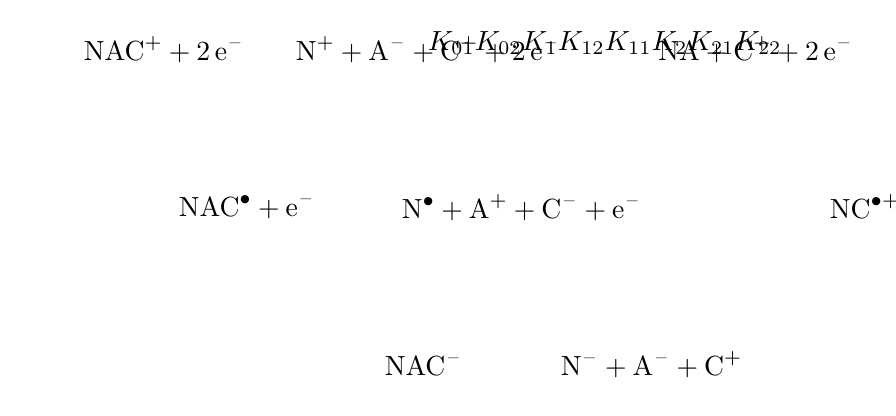
\begin{tikzpicture}[node distance=2cm]
		\node (N1) {\ce{N+ + A- + C+ + 2e-}};
		\node[right=1cm of N1] (N1c) {\ce{NA + C+ + 2e-}};
		\arrwy{N1.east}{N1c.west}{$K_{01}$}
		\node[left=1cm of N1] (N1cc) {\ce{NAC+ + 2e-}};
		\arrwy{N1cc.east}{N1.west}{$K_{02}$}
		
		\node[below of = N1] (N2) {\ce{N^. + A+ + C- + e-}};
		\arrwx{N1.south}{N2.north}{$K_{1}$}
		\node[below of=N1cc] (N2cc) {\ce{NAC^. + e-}};
		\arrwy{N2cc.east}{N2.west}{$K_{12}$}
		\node[below of=N1c] (N2c) {\ce{NC^.+ + A- + e-}};
		\arrwy{N2.east}{N2c.west}{$K_{11}$}
		
		\node[below of=N2] (N3) {\ce{N- + A- + C+}};
		\arrwx{N2.south}{N3.north}{$K_2$}
		\node[right= 2cm of N3] (N3c) {\ce{NC  + A-}};
		\arrwy{N3.east}{N3c.west}{$K_{21}$}
		\node[below of=N2cc] (N3cc) {\ce{NAC-}};
		\arrwy{N3cc.east}{N3.west}{$K_{22}$}
	\end{tikzpicture}
	\caption{Scheme illustrating the different possible reactions: \ce{N+} and \ce{N-} are the oxidized and reduced forms of a given nitroxide, \ce{N^.}, and \ce{C+} and \ce{A-} are the countercation and anion coming from electrolyte, respectively. Horizontal arrows are ion-pairing reactions (with the \ce{AC} pair in left, with a single counterion in right), while vertical arrows are electrochemical reactions.}
	\label{fig:cip}
\end{figure}

Following Mugisa and co-workers \cite{mugisaEffectIonparingKinetics2024}, a quantitative model is derived from Fig.~\ref{fig:cip}, owing that: \begin{inparaenum}[(i)]
	\item the total concentration of redox-active species is given by $c_{ox} = [\ce{N+}] + [\ce{NA}] + [\ce{NAC+}]$, $c_{rad} = [\ce{N^.}] + [\ce{NAC^.}]$, and $c_{red} =  [\ce{N-}] + [\ce{NC}] + [\ce{NAC-}]$,
	\item due to electroneutrality, $ [\ce{C+}] = [\ce{A-}] $,
	\item the electrolyte is present in large amounts compared to redox-active species, hence $[X] = [\ce{C+}] = [\ce{A-}] $ is constant ($[X]$ represents the electrolyte concentration),
	\item at the equilibrium of redox reactions, $c_{ox} = c_{rad}$ ($K_1$) and $c_{red} = c_{rad}$ ($K_2$), and
	\item the redox potentials of the ion-pair complexes are smaller than the one of the free species.
\end{inparaenum}
Within these assumption, the following electrolyte concentration-dependent (formal) redox potentials are obtained:\begin{align}
	E^f_{abs}(\ce{N+|N^.}) &= E^0_ {abs}(\ce{N+|N^.})+\frac{RT}{F}\,\ln\left[\frac{1+K_{11}\,[X]+K_{12}\,[X]^2}{1+K_{01}\,[X]+K_{02}\,[X]^2}\right],\\
	E^f_{abs}(\ce{N^.|N-}) &= E^0_ {abs}(\ce{N^.|N-})+\frac{RT}{F}\,\ln\left[\frac{1+K_{21}\,[X]+K_{22}\,[X]^2}{1+K_{11}\,[X]+K_{12}\,[X]^2}\right],
\end{align}
in which $K_{ij}= \exp\left[-\frac{\Delta G_{cplx}^\star}{RT}\right]$, where $\Delta G_{cplx}^\star$ is the free Gibbs energy change [computed with Eq.~\eqref{eq:gtot}] for a given complexation reaction.

An example is provided in Fig.~S2: while $K_{(i+1)1} / K_{i1}$ ($i\in[0,1]$) governs the behavior at low $[X]$, the trend at high $[X]$ is determined by $K_{(i+1)2} / K_{i2}$.\todo{now, it is not that simple ;)}

\subsection{Model for the ion-pair formation}

Insight into the formation of ion pairs ($K_{01}$ and $K_{21}$ in Fig.~\ref{fig:cip}) is provided by a simple model proposed by Lund et al. \cite{lundDielectricInterpretationSpecificity2010}. It is based on the balance between the solvation of the individual charges (described by the Born model, Eq.~\eqref{eq:born}) and the formation of a dipole when the two charges interact, leading to the famous Onsager model \cite{onsagerElectricMomentsMolecules1936,krishtalikElectrostaticIonSolvent1991,aubretUnderstandingLocalField2019}. From the thermodynamic cycle given in Fig.~\ref{fig:ionpair}, one can derive the following expression: \begin{equation}
	\Delta G_{\text{pair}}^\star = \frac{1}{4\pi\varepsilon_0}\,\left\{\left[\frac{q_1^2}{2a_1}+\frac{q_2^2}{2a_2}\right]\,\left[1-\frac{1}{\varepsilon_r}\right]+\frac{q_1\,q_2\,|q_1-q_2|}{2\,\mu}-\frac{\varepsilon_r-1}{2\varepsilon_r+1}\,\frac{\mu^2}{a^3}\right\},\label{eq:pair}
\end{equation}
where $a_1$, $a_2$, and $a=s_2\,( a_1^3+a_2^3)^{1/3}$ are the radii of the cavities corresponding to $q_1$, $q_2$, and the dipole, respectively, defined as $\mu = \frac{s_1}{2}\,|q_2-q_1|\,(a_1+a_2)$.  $s_1$ and $s_2$ are scaling factors, which account for the electrostatic attraction between the two charges forming the dipole ($s_1\leq 1$) and the fact that the cavity might not be spherical ($s_2\geq 1$).

\begin{figure}[!h]
	\centering
	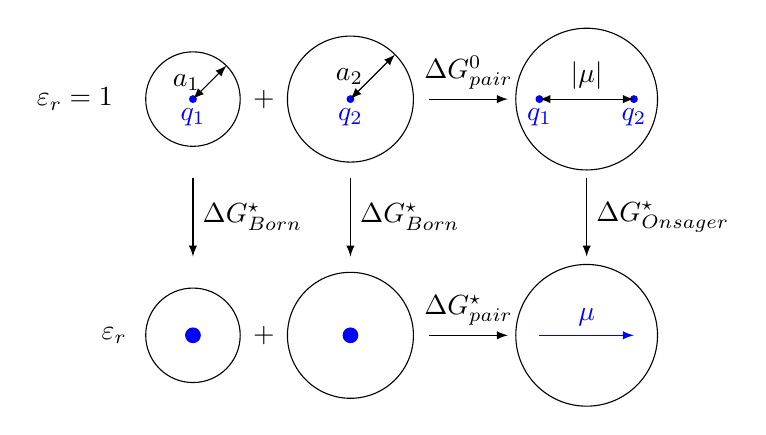
\begin{tikzpicture}
		\draw (-1.5,0) node{$\varepsilon_r=1$};
		\draw (-1,-3) node{$\varepsilon_r$};
		\draw (0,0) circle (.6cm);
		\fill[blue] (0,0) node[below]{$q_1$}  circle (.05cm);
		\draw[latex-latex] (0,0) -- (45:0.6) node[midway,left]{$a_1$};
		
		\draw (.9,0) node{+};
		
		\draw (2,0) circle (.8cm);
		\fill[blue] (2,0) node[below]{$q_2$}  circle (.05cm);
		\draw[latex-latex] (2,0) -- +(45:0.8) node[midway,left]{$a_2$};
		
		\draw[-latex] (3,0) -- +(1,0) node[midway,above]{$\Delta G^0_{pair}$};
		
		\draw (5,0) circle (.9cm);
		\fill[blue] (4.4,0) node[below]{$q_1$} circle (.05cm);
		\fill[blue] (5.6,0) node[below]{$q_2$}  circle (.05cm);
		\draw[latex-latex](4.4,0) -- (5.6,0) node[midway,above]{$|\mu|$};
		
		\draw[-latex] (0,-1) -- +(0,-1) node[midway,right]{$\Delta G^\star_{Born}$};
		\draw[-latex] (2,-1) -- +(0,-1) node[midway,right]{$\Delta G^\star_{Born}$};
		\draw[-latex] (5,-1) -- +(0,-1) node[midway,right]{$\Delta G^\star_{Onsager}$};
		
		\fill[blue] (0,-3) circle (.1cm);
		\draw (0,-3) circle (.6cm);
		
		\draw (.9,-3) node{+};
		
		\draw (2,-3) circle (.8cm);
		\fill[blue] (2,-3) circle (.1cm);	
		
		\draw[-latex] (3,-3) -- +(1,0) node[midway,above]{$\Delta G^\star_{pair}$};
		
		\draw (5,-3) circle (.9cm);
		\draw[-latex,blue](4.4,-3) -- (5.6,-3) node[midway,above]{$\mu$};
	\end{tikzpicture}
	\caption{Thermodynamic cycle for the formation of ion-pair, adapted from Ref.~\citenum{lundDielectricInterpretationSpecificity2010}.}
	\label{fig:ionpair}
\end{figure}

This qualitative model (see Fig.~S3) indicates that ion pairing depends on: \begin{inparaenum}[(i)]
	\item the ratio $\chi = a_1 / a_2$, with $\chi \sim 1$ leading to the lowest pair formation energy (as previously noted by Lund and colleagues),
	\item the attraction between the charges ($s_1$),
	\item the shape of the final cavity (pairing energy increases with $s_2$), and
	\item the dielectric constant $\varepsilon_r$.
\end{inparaenum}
While the latter parameter has only a minor influence (although the difference increases with $s_1$), the formation of a pair of ions is favored in less polar solvents, as expected.\todo{Le modele est intéréssant pour les liquides ioniques, soit dit en passant. D'ailleurs, est ce que c'est en ligne avec ce que le papier de 2019 dit?}


\subsection{Counterion as a fictitious particle}

Alternatively, Matsui et al. \cite{matsuiDensityFunctionalTheory2013} proposed that the impact of counterions on the redox potential of $X^z$ could be described using a single fictitious particle, $P^{-z}$, with a radius $a=fa_0$ proportional to that of the redox species, $a_0$ (considered constant for all oxidation states of $X$), and bearing the appropriate counter-charge, $-z$. They suggested evaluating the energy of this particle using a modified Born approach [Eq.~\eqref{eq:born}]:\begin{align}
	&\Delta G^\star_{P}(P^z) = \frac{1}{4\pi\epsilon_0}\, \frac{q^2}{2fa_0}\,\left[\frac{1}{\varepsilon_r}-1\right]\,\erf(\mu\,a_0\,|q|),
\end{align}
where $f$ and $\mu$ are method-dependent factors, the latter being described in Ref.~\cite{matsuiDensityFunctionalTheory2013} as a screening factor.


In the presence of this fictitious particle, the reduction of $X^z$ becomes:\begin{equation*}
	\begin{array}{rl}
		X^z + n_e\,e^- &\rightarrow X^{z-n_e} \\
		P^{-z} \phantom{ + n_e\,e^-} &\rightarrow P^{n_e-z} + n_e\,e^- \\
		\hline
		X^z + P^{-z}&\rightarrow X^{z-n_e} +P^{n_e-z}\\
	\end{array}  \label{eq:corr}
\end{equation*}
and therefore,\begin{align}
	E^p_{abs}(X^z|X^{z-n_e}) &= 	E_{abs}^0(X^{z}|X^{z-n_e}) -\frac{1}{n_e\,F}\,[\Delta G^\star_{P}(P^{n_e-z}) - \Delta G^\star_{P}(P^{-z})] \nonumber\\
	&= 	E_{abs}^0(X^{z}|X^{z-n_e}) -\frac{\Delta\Delta G^\star_P}{n_e\,F}, \label{eq:matsui} 
\end{align}
where:\begin{align*}
	\Delta\Delta G^\star_P&=\frac{1}{4\pi\epsilon_0}\frac{1}{2fa_0}\,\left[\frac{1}{\varepsilon_r}-1\right]\times\nonumber\\
	&\left[ (n_e-q)^2\,\erf(\mu\,a_0\,|n_e-q|)-q^2\,\erf(\mu\,a_0\,|q|)\right].
\end{align*}
Matsui and co-workers propose to  find the parameter $f$ and $\mu$ that minimize the difference between $E^p_{rel}(X^z|X^{z-n_e})$  [from Eq.~\eqref{eq:ecalc}] and the experimental $E^0_{rel}(X^z|X^{z-n_e})$.  Note that they therefore considers that $ E^{0}_{abs}(\text{SHE})$ is a third fitting parameter.

\section{Methodology} \label{sec:methodo}

In this study, the set of nitroxides considered by Hogsdon \textit{et al.} (compounds \textbf{1}-\textbf{54}) is examined, supplemented with a few additional compounds for completeness (\textbf{55}-\textbf{61}). All structures are depicted in Fig.~\ref{fig:nitroxides}. The \ce{AC} pair, consisting of \ce{BF4^-} (\ce{A-}) and \ce{NMe4^+} (\ce{C+}), is used as the electrolyte.


\begin{figure}[!p]
\centering
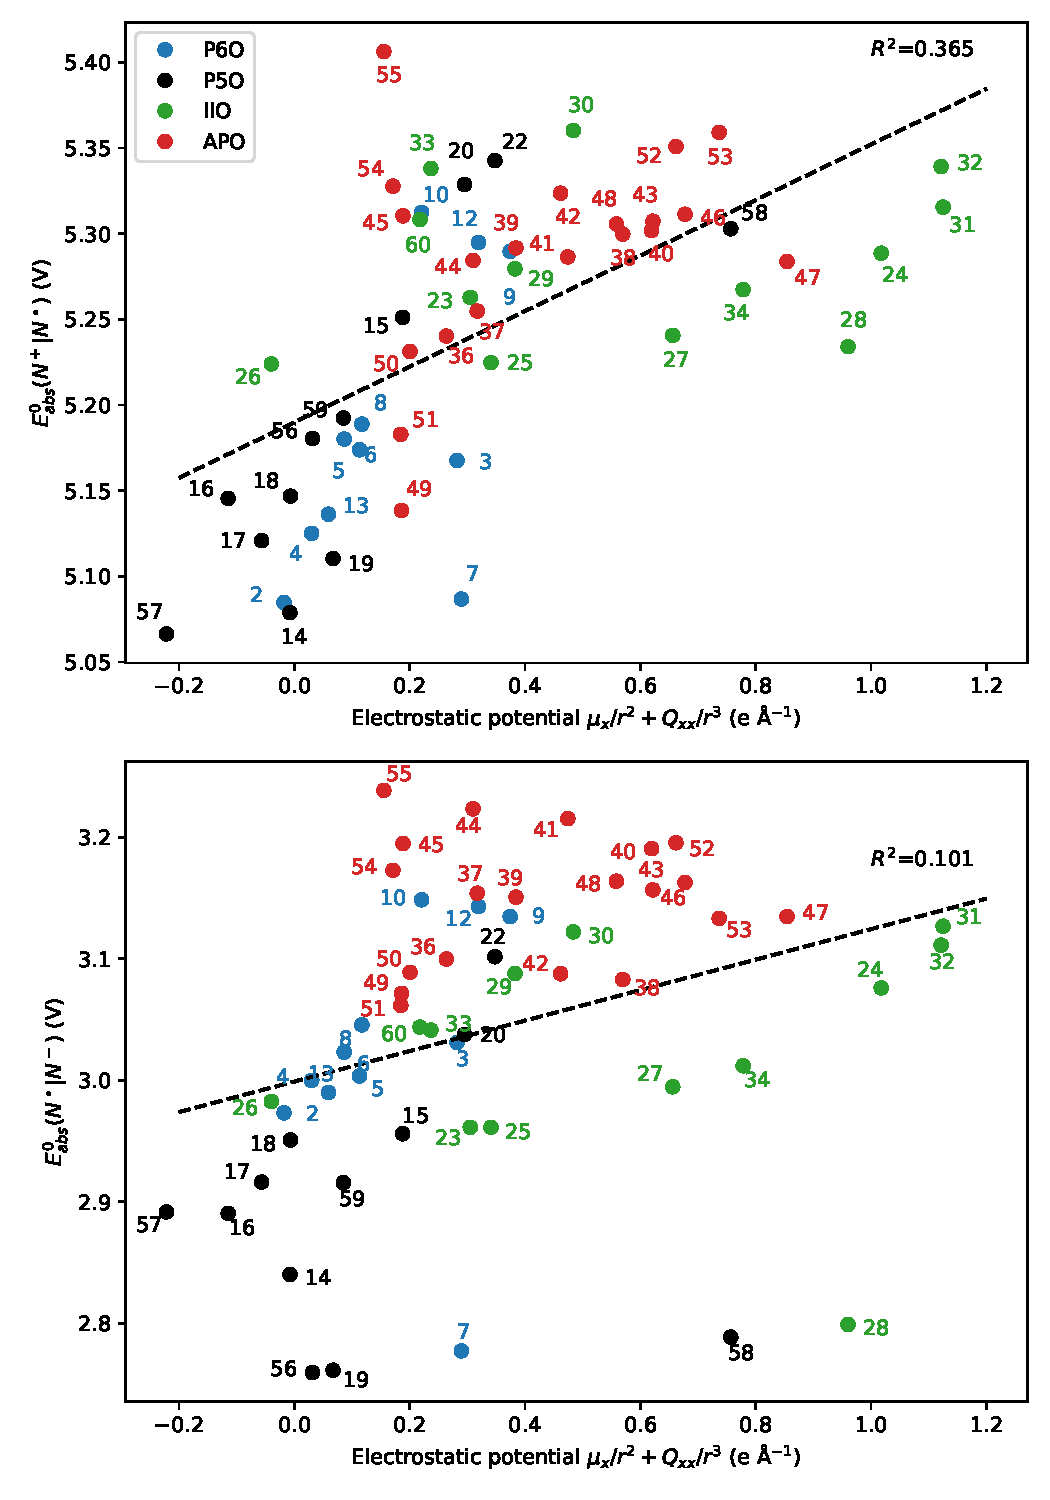
\includegraphics[width=\linewidth]{Figure6}
\caption{The different nitroxides considered in this work, sorted by families. Compounds \textbf{1}-\textbf{54} are from Ref.~\citenum{hodgsonOneElectronOxidationReduction2007}, while compounds \textbf{55}-\textbf{61} where considered for completeness. Experimental (reduction or oxidation) potentials are available in water if the number is written in red, while they are available in acetonitrile if the number is underlined.}
\label{fig:nitroxides}
\end{figure}

Geometry optimizations and subsequent vibrational frequency calculations were performed at the $\omega$B97X-D/6-311+G(d) level in water and acetonitrile (described using the SMD \cite{marenichUniversalSolvationModel2009} approach) with Gaussian 16 C02 \cite{g16}. For compound \textbf{1}-\textbf{54}, the geometries obtained by Hodgson et al. \cite{hodgsonOneElectronOxidationReduction2007} have been used as a starting point, taking advantage of their extensive conformational search. All radical forms are considered to have a doublet ground state. Then, the same calculations were preformed in acetonitrile for the subset of compounds for which experimental redox potentials are available (listed in Fig.~\ref{fig:nitroxides}). Finally, to study the influence of the substituent on the redox potential, following Zhang and co-workers \cite{zhangEffectHeteroatomFunctionality2018}, single point calculation are performed at the $\omega$B97X-D/6-311+G(d) level in gas phase, using the optimized geometries of  the radical states of each nitroxides (in water) in which $>$\ce{N-O^.} moiety is substituted by \ce{CH_2} (the rest of the geometry is kept fixed).

Since all thermochemical quantities are $\kappa$-dependent, analyses were performed using custom Python scripts. When required (e.g., in Eq.~\eqref{eq:dh}), the value of $a$ (the radius of the solute cavity) is taken as half the largest distance between two atoms in the molecule. Furthermore, a value of $\varepsilon_{r,wa}=80$ for water and $\varepsilon_{r,ac}=35$ for acetonitrile is used. These relative permittivities correspond to those of the pure solvents and are known to be lower in the respective electrolyte solutions \cite{silvaTrueHuckelEquation2022}. These variations can be substantial; for example, $\varepsilon_r \approx 70$ for a solution containing \SI{1}{\mol\per\kilo\gram} of \ce{NaCl} in water \cite{kontogeorgisDebyeHuckelTheoryIts2018, silvaTrueHuckelEquation2022}, but they depend on the nature of the electrolyte.
Unless otherwise mentioned, the value of $\kappa^2$ is obtained assuming  $c_{ox} = c_{rad} = c_ {red} = \SI{1e-3}{\mole\per\liter}$, a prototypical concentration in measurements.

\clearpage

\section{Results and discussion} \label{sec:results}

\subsection{Structure-activity relationships} \label{sec:sar}


Oxidation and reduction potentials of nitroxide radicals in water, grouped by family, are plotted in Fig.~\ref{fig:family} (see also Table S1). Compared to \textbf{1}, modifying the molecular structure or adding substituents generally increases both the oxidation and reduction potentials. Regarding structural impacts, six-membered ring compounds (P6O and APO) exhibit higher reduction potentials than their five-membered ring counterparts (P5O and IIO). Additionally, the incorporation of one or two aromatic rings (IIO and APO) enhances both the oxidation and reduction potentials.


\begin{figure}[!h]
	\centering
	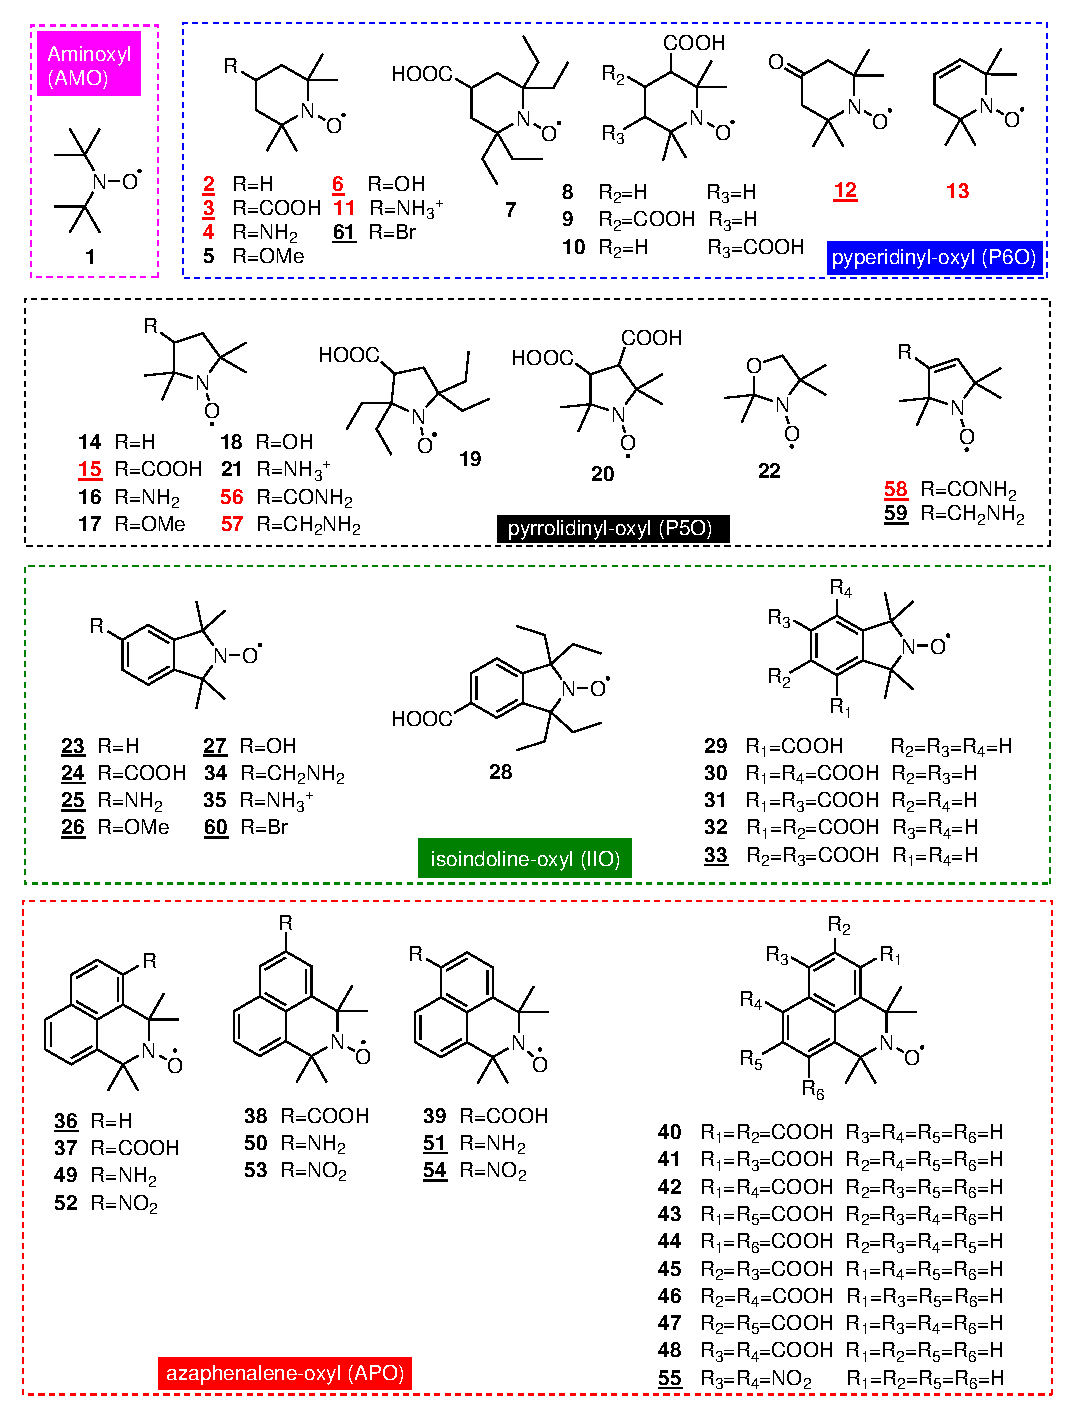
\includegraphics[width=.9\linewidth]{Figure7}
	\caption{Relationship between absolute oxidation and reduction potentials of nitroxides, as computed at the $\omega$B97X-D/6-311+G(d) level in water (SMD), with $[\ce{X}]=\SI{0}{\mole\per\liter}$. The color indicate the family (Fig.~\ref{fig:nitroxides}). For each of them, an ellipse is drawn, centered on the mean potential value among the family, and which width and height are given by the standard deviations.}
	\label{fig:family}
\end{figure}

Regarding the impact of substituents, it is noteworthy that non-substituted nitroxides within each family (\textit{i.e.}, \textbf{2}, \textbf{14}, \textbf{23}, and \textbf{36}) generally have some of the lowest oxidation and reduction potentials within their respective groups. Several trends emerge based on the nature of the substituent: \begin{inparaenum}[(i)]
	\item shielding the radical center with ethyl groups instead of methyl groups (\textbf{7}, \textbf{19}, and \textbf{28}) results in a decrease in potentials (particularly the reduction potential), likely due to changes in inductive effects,
	\item protonation of \ce{NH2} increases the potentials, especially in P5O,
	\item multiple substitutions by COOH (\textit{e.g.}, \textbf{8} vs. \textbf{9} and \textbf{10}) also increase the potentials, though the effect is less pronounced in IIO and APO,
	\item compounds with mesomeric donor substituents (\ce{NH2}, \ce{OH}, \ce{OMe}) have lower potentials than those with acceptor substituents (COOH, \ce{NO2}), particularly in aromatic systems (IIO and APO), and
	\item compounds \textbf{56} and \textbf{58} have surprisingly low reduction potentials.
\end{inparaenum}
As a consequence, \textbf{55} exhibits the highest oxidation and reduction potentials among all the compounds studied in this paper.


To elucidate these effects, attempts were made to correlate both potentials with Hammett constants for P5O and P6O, but the correlations were found to be very weak, especially for reduction (see Fig.~S4). The electrostatic interaction model [Eq.~\eqref{eq:Er}] provides more insights. Results are presented in Fig.~\ref{fig:corr} (see also Table S3). However, this model fails to account for the effect of substituting methyl groups with ethyl groups. Moreover, including the disubstituted compounds (e.g., \textbf{9}) worsens the correlation ($R^2 \sim 0.5$ and 0.3 for oxidation and reduction, respectively). Compounds \textbf{56} and \textbf{58} remain outliers for reduction. Therefore, all three sets of compounds were treated as outliers.
On the positive side, this model helps explain some of the effects mentioned above: the increase in oxidation (and reduction) potential for aromatic compounds correlates with an increase in quadrupole moment ($Q_{xx} > \SI{5}{\elementarycharge\bohr\squared}$ for most member of IIO or APO), while the modification due to donor/acceptor substituents is linked to changes in the dipole moment. For example, aromatic compounds that have \ce{NH2} has substituent (\textit{e.g.}, \textbf{51}) are characterized by  $\mu_{x} < 0$, which gets larger for coumpounds have \ce{COOH} (\textit{e.g.}, \textbf{39}) or \ce{NO2} (\textit{e.g.}, \textbf{54}). It also accounts for some effects due to the position of the substituent (see, e.g., \textbf{49}-\textbf{51}), which was not the case with the original model by Zhang and co-workers (resulting in weak correlations, $R^2 \leq 0.3$).
Finally, although it is not directly applicable to charged substituents (\textbf{11}, \textbf{21}, and \textbf{35}), for which the multipole moments are ill-defined, the leading term $q/r$ would result in a positive contribution to $E_r$, which correlates well with the increase in oxidation and reduction potential for these compounds.


\begin{figure}[!h]
\centering
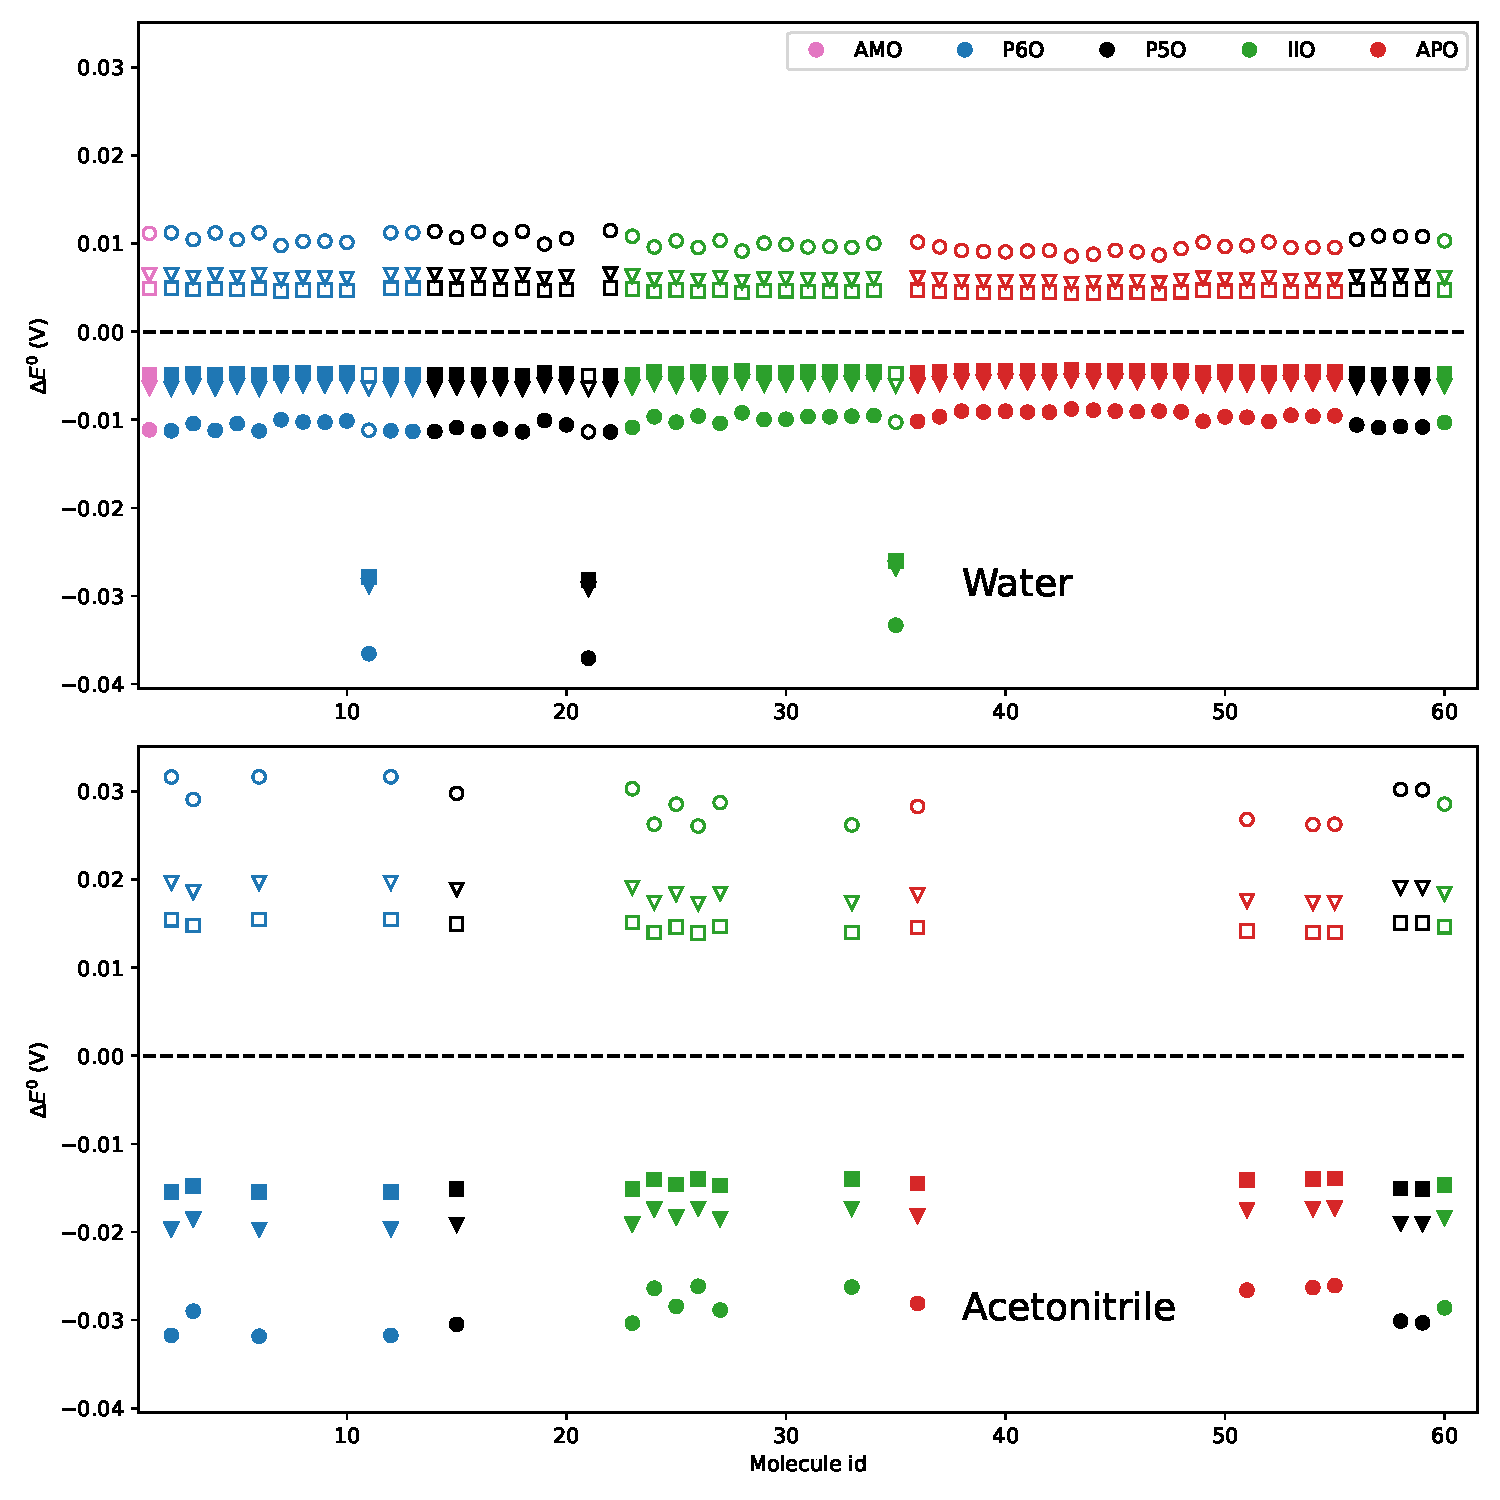
\includegraphics[width=\linewidth]{Figure8}
\caption{Relationship between absolute oxidation (top) and reduction (bottom) potentials of nitroxides and the electrostatic potential between the redox center ($>$\ce{N-O^.}) and the substituent, as computed at the $\omega$B97X-D/6-311+G(d) level in water (SMD), with $[\ce{X}]=\SI{0}{\mole\per\liter}$. Triangular marker ($\blacktriangle$) indicates results that are excluded from the correlation (see text).}
\label{fig:corr} 
\end{figure}

\clearpage

\subsection{Impact of the solvent} \label{sec:solv}

The difference between redox potentials computed in water and acetonitrile is illustrated in Fig.~\ref{fig:watvsac} (see also Table S2): except for compound \textbf{12}, the oxidation potential is only minimally affected, while there is a disparity of greater than \SI{0.5}{\volt} for the reduction potentials. In first approximation, the Born model [Eq.~\eqref{eq:born}] can account for these findings: for oxidation, the change in potentials in the two solvents, $E^0_{ac} - E^0_{wa}$, is proportional to $\varepsilon_{r,ac}^{-1}-\varepsilon_{r,wa}^{-1}$, which is positive (assuming that \ce{N^.} is neutral, which holds true for the subset of compounds considered here), whereas for reduction, it is proportional to $\varepsilon_{r,wa}^{-1}-\varepsilon_{r,ac}^{-1}$, which is negative. Since this impact is systematic, similar trends (in terms of the impact of substituents) between redox potentials in water and acetonitrile are observed.


\begin{figure}[!h]
	\centering
	\includegraphics[width=\linewidth]{Figure9}
	\caption{Comparison between absolute oxidation (left) and reduction (right) potentials of nitroxides as computed at the $\omega$B97X-D/6-311+G(d) level in water and acetonitrile (SMD), with $[\ce{X}]=\SI{0}{\mole\per\liter}$. The dashed line represents no change. }
	\label{fig:watvsac}
\end{figure}

\subsection{Impact of the electrolytes} \label{sec:elect}

So far, the concentration of electrolyte, $[X]$, has been maintained at zero. To evaluate its impact on the redox potentials, the DH correction itself is initially examined in Fig.~\ref{fig:DH}. As anticipated, it remains small within the concentration range considered here (a few hundredths of millivolts for $[X] \leq \SI{1}{\mole\per\liter}$ and larger in acetonitrile), increasing with $[X]$. Its sign differs between oxidation and reduction potentials. Additionally, it is diminished for compounds belonging to the IIO and APO families (as they are larger molecules with larger $a$), but amplified for species with a net positive charge (\textbf{11}, \textbf{21}, \textbf{35}), for which the correction for oxidation and reduction potentials is negative.


\begin{figure}[!h]
	\centering
	\includegraphics[width=\linewidth]{Figure10}
	\caption{Impact of the Debye-Huckel correction, as $\Delta E^0 = -\frac{\Delta \Delta G_{DH}^\star}{F}$ for $[X]=\SI{1}{\mole\per\liter}$ (round markers), $[X]=\SI{0.1}{\mole\per\liter}$ (triangular markers, $\blacktriangle$)  and $[\ce{X}]=\SI{0}{\mole\per\liter}$ (square markers, $\blacksquare$), as computed at the $\omega$B97X-D/6-311+G(d) level in water (top) and acetonitrile (bottom) using SMD. Filled (empty) markers represent the correction to the oxidation (reduction) potential. }
	\label{fig:DH}
\end{figure}

Next, the formation of ion pairs is addressed. First, the complexation equilibrium constants between the oxidized and reduced states (which bear a formal charge, except for \textbf{11}, \textbf{21}, and \textbf{35}) and a counterion are reported in Fig.~\ref{fig:Kx1} (see also Tables S4-S5 and Fig.~S6). In water and acetonirile, the equilibrium constant $K_{01}$ (between \ce{N+} and $\ce{A-}$) is approximately \num{e-4} ($\Delta G^\star_{cplx} \sim \SI{25}{\kilo\joule\per\mole}$), indicating unfavorability complexation. Then, on the one hand, $K_{21}$ (between \ce{N-} and $\ce{C+}$) is generally smaller (especially for members of P6O) in water, except in a few cases. This contradicts the electrostatic model for ion pair formation [Eq.~\eqref{eq:pair}], which predicts $K_{21} > K_{01}$, as it favors pairs composed of ions of similar size. In this study, \ce{NMe4+} has a larger radius (\SI{2.1}{\angstrom}) than \ce{BF4-} (\SI{1.5}{\angstrom}), the former being closer to the size of nitroxides ($>$\SI{3}{\angstrom}). On the other hand, the results in acetonitrile follow the prediction of the model, with $K_{21} \sim \num{e-2}$.


\begin{figure}[!h]
\centering
\includegraphics[width=\linewidth]{Figure11}
\caption{Value of the complexation equilibrium constants $K_{01}$ (round markers, $\bullet$) and $K_{21}$ (square markers, $\blacksquare$), as computed at the $\omega$B97X-D/6-311+G(d) level in water (top) and acetonitrile (bottom) using SMD and $[X]=\SI{1}{\mole\per\liter}$.  The dashed line is there to help visualization. }
\label{fig:Kx1}
\end{figure}

A closer examination of Fig.~\ref{fig:Kx1} reveals that compounds of the P6O family exhibit distinct behavior, particularly in terms of the interaction between the aminoxyl group and the cation. This interaction is notably weaker ($\Delta G^\star_{cplx} > \SI{40}{\kilo\joule\per\mole}$) in water compared to other families. This can be elucidated by analyzing the geometries of the ion pairs. 
Firstly, it should be noted that within the P6O family, where the basic skeleton is a cyclohexane, the \ce{N+=O} group occupies an equatorial position while the \ce{N-O-} bond adopts an axial position. The presence of nearby methyl groups hinders electrostatic interaction, especially for bulky counterions. This effect is less pronounced in other families, where the skeleton prevents the oxygen from adopting such a position (particularly in IIO and APO).
Then,  it is observed that there are two possible positions for the counterion: 
\begin{inparaenum}[(i)]
	\item near the redox center ($>$\ce{N-O^.}), ``in front" of the methyl groups, and 
	\item near the substituent, ``behind" the methyl groups.
\end{inparaenum}
Using compound \textbf{4} as an example (see Fig.~\ref{fig:pos-anion}), the energy difference between these positions is small (approximately \SI{5}{\kilo\joule\per\mole} for \textbf{12}). The first position is generally favored. In acetonitrile, however, the nitroxide-to-counterion distance is smaller due to the lower dielectric constant, which results in reduced charge screening. Consequently:
\begin{inparaenum}[(i)]
	\item for the oxoammonium ion, the lower charge screening in acetonitrile secludes the \ce{BF4-} from interacting with the substituent in the second position, favoring the first position, and
	\item for hydroxylamine, both positions result in smaller complexation energies due to the reduced dielectric constant.
\end{inparaenum}
\todo{What about the other families?} 


\begin{figure}[!h]
	\centering
	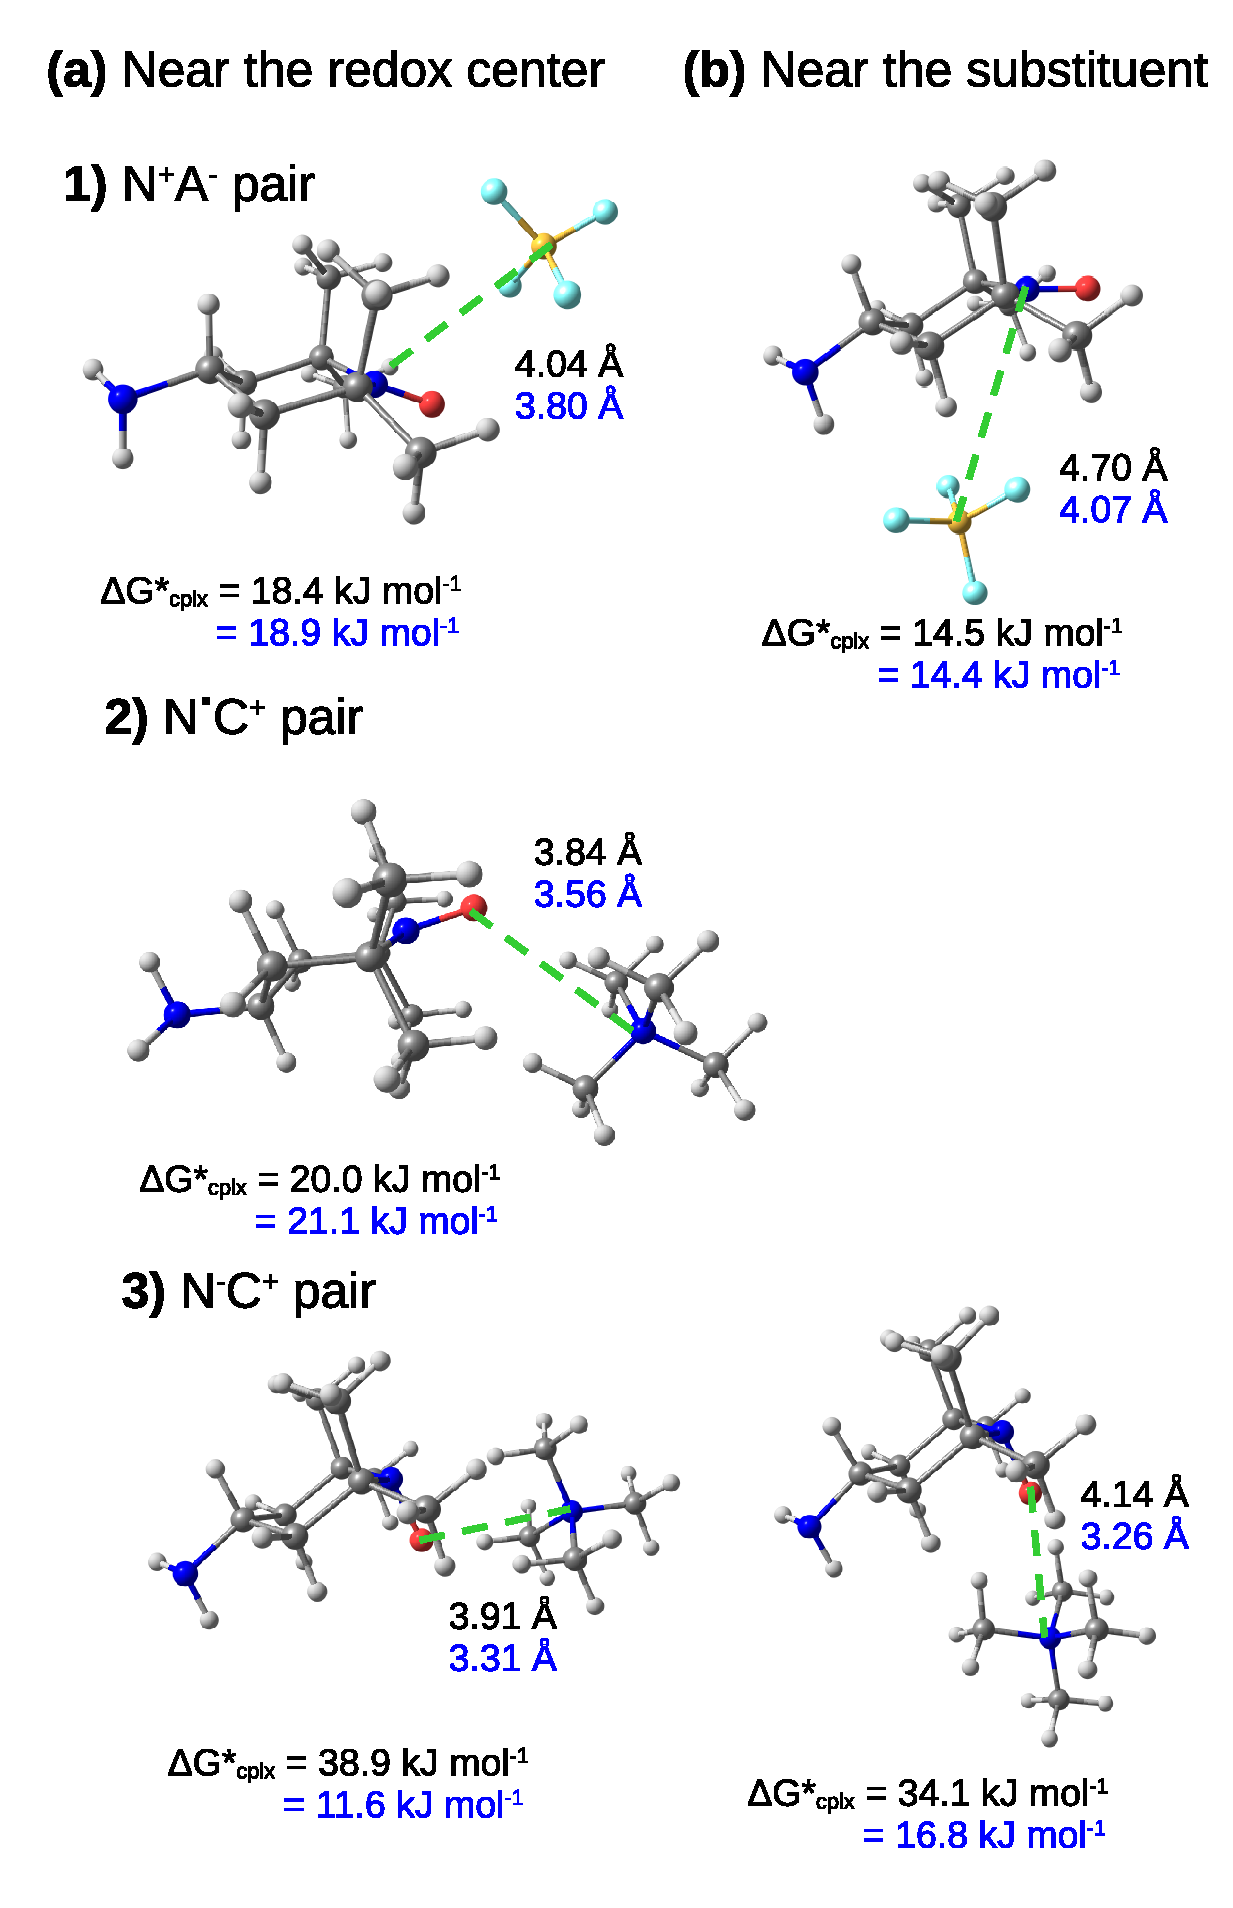
\includegraphics[width=.7\linewidth]{Figure12}
	\caption{Impact of the counterion position (a) or (b) on the distance between the counterion and the redox center (the nitrogen in the oxidized form, $>$\ce{N+=O}, or the oxygen in the reduced form, $>$\ce{N-O-}), and on $\Delta G^\star_{cplx}$, using compound \textbf{4} as an example. Calculations were performed at the $\omega$B97X-D/6-311+G(d) level in water (black) and acetonitrile (blue).}
	\label{fig:pos-anion}
\end{figure}


Finally, complexation to the \ce{AC} pair is considered (Fig.~\ref{fig:Kx2}, Tables S6-S7). As expected, the equilibrium constants are smaller (by about four order of magnitude, $\Delta G^\star_{cplx} \sim \SI{50}{\kilo\joule\per\mole}$) than the ones that were previously discussed.\todo{How does that compares to \citenum{wylieImprovedPerformanceAllOrganic2019a}? Structure-activity relationships?}


\begin{figure}[!h]
\centering
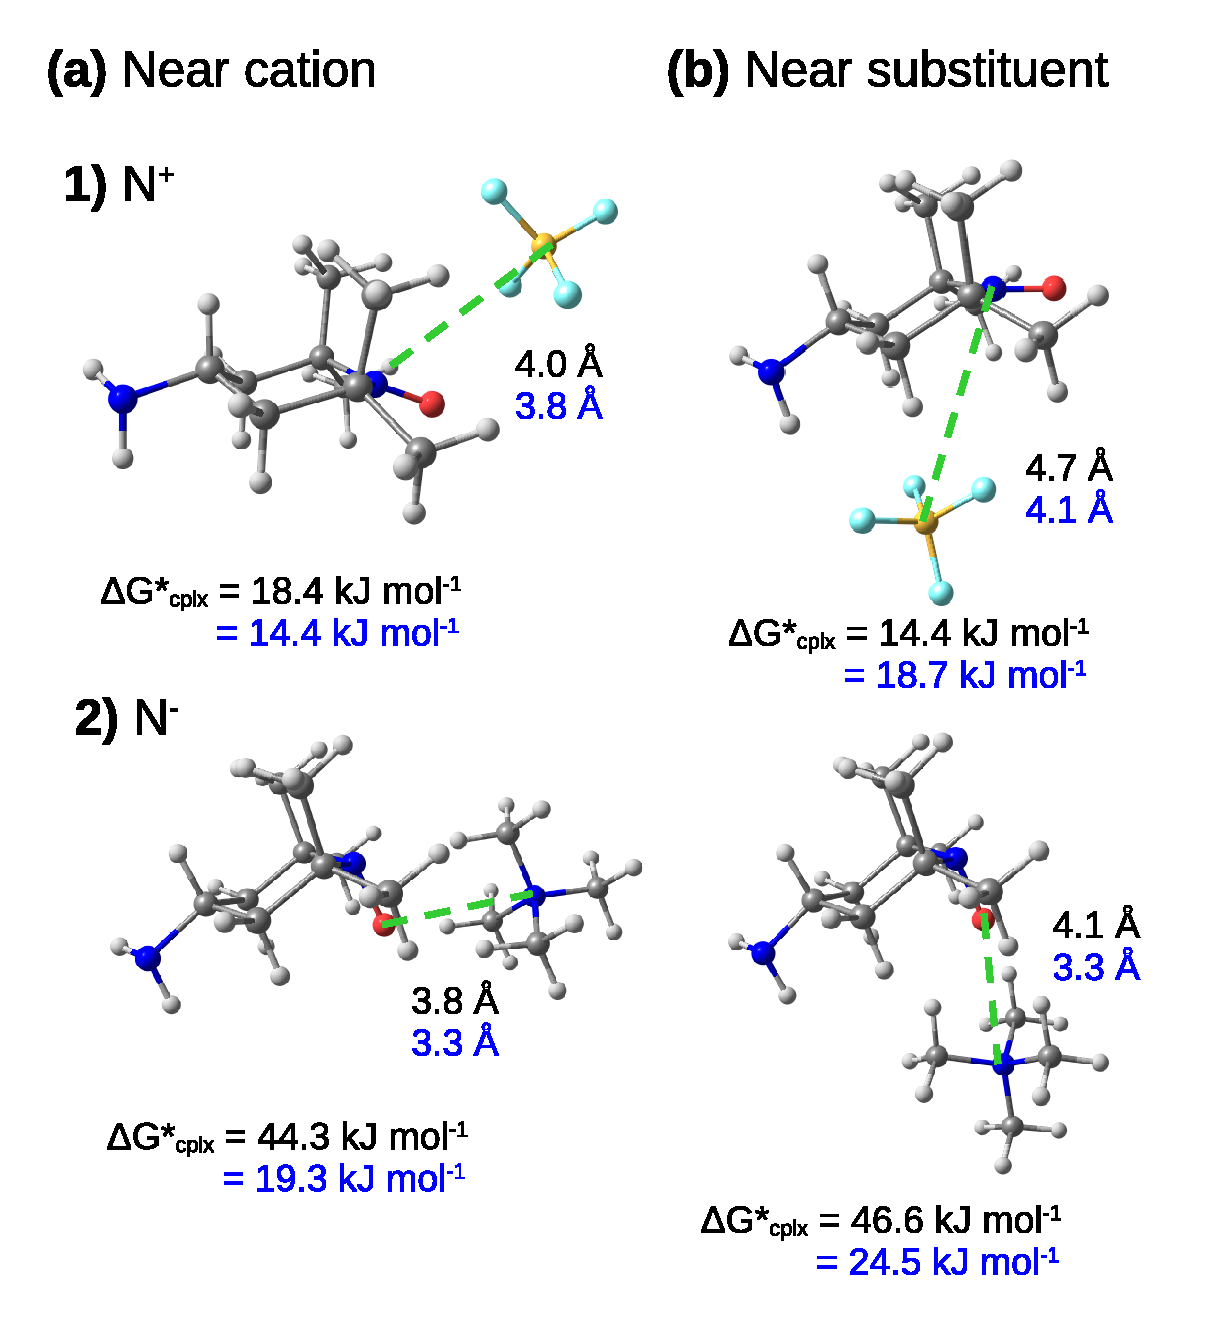
\includegraphics[width=\linewidth]{Figure13}
\caption{Value of the complexation equilibrium constants $K_{02}$ (round markers, $\bullet$), $K_{12}$ (triangular markers, $\blacktriangle$) and $K_{22}$ (square markers, $\blacksquare$) for the 3 oxidation state of nitroxides, as computed at the $\omega$B97X-D/6-311+G(d) level in water (top) and acetonitrile (bottom) using SMD and $[X]=\SI{1}{\mole\per\liter}$.  The dashed line is there to help visualization. }
\label{fig:Kx2}
\end{figure}

\clearpage
\subsection{Comparison to experiment} \label{sec:exp}

\begin{itemize}
	\item So one can drop $K_{x2}$,
	\item Impact is small, isn't?
	\item What about Matsui?
\end{itemize}

\clearpage
\section{Conclusion} \label{sec:conclusion}

Random thoughts:\begin{itemize}
	\item more of DH could be included (dipole, quandrupole)
	\item We only focused on the impact of substituent. Other study do the counterion part.
	\item The impact remains moderate, but I hope I have provided keys in understanding interaction.\todo{check \cite{zhangInteractionsImidazoliumBasedIonic2016}}
	\item Ionic liquids needs to be addressed at some point ;)
\end{itemize}
	
	
\bibliographystyle{elsarticle-num-names} 
\bibliography{biblio}
	
\end{document}
\endinput
%%
%% End of file `elsarticle-template-num.tex'.
